% Source: Code/xband-radar-sim/docs/radar_simulation_technical.tex
% Description: Effect of beam spreading convolution. Thin radial artifacts become realistic blob-shaped returns matching the antenna beamwidth.

\documentclass[border=4pt]{standalone}
\usepackage{algpseudocode}
\usepackage{amsmath,amssymb,amsfonts}
\usepackage[T1]{fontenc}
\usepackage{graphicx}
\usepackage{pgfplots}
\usepackage{tikz}
\usepackage{xcolor}
\pgfplotsset{compat=1.18}
\usetikzlibrary{arrows.meta,positioning,shapes.geometric,calc,patterns,decorations.pathmorphing,3d,angles,quotes}

\definecolor{radargreen}{RGB}{0,255,0}
\definecolor{raycolor}{RGB}{255,165,0}
\definecolor{targetcolor}{RGB}{255,0,0}
\definecolor{groundcolor}{RGB}{139,90,43}
\definecolor{skycolor}{RGB}{135,206,235}
\definecolor{beamcolor}{RGB}{255,255,0}


\begin{document}
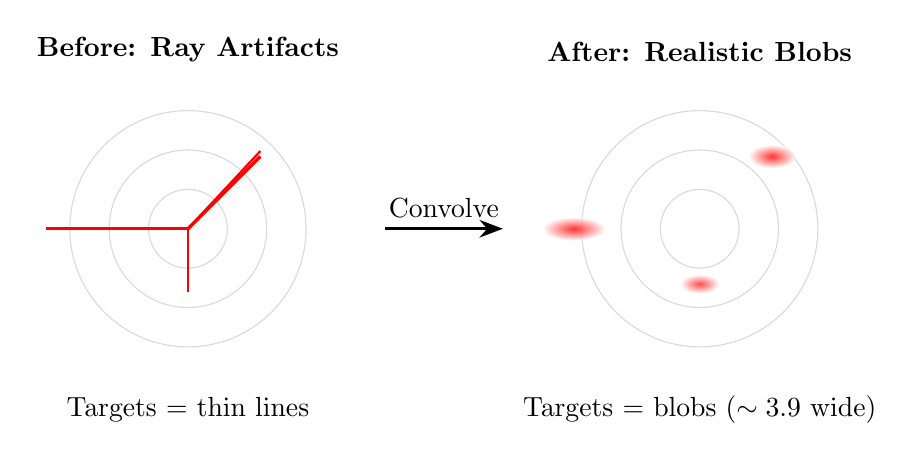
\begin{tikzpicture}
    % Before
    \begin{scope}[shift={(0,0)}]
        \node[above] at (2,4) {\textbf{Before: Ray Artifacts}};

        % Polar grid
        \draw[gray!30] (2,2) circle (1.5);
        \draw[gray!30] (2,2) circle (1);
        \draw[gray!30] (2,2) circle (0.5);

        % Thin radial lines (artifacts)
        \draw[red, very thick] (2,2) -- ++(45:1.3);
        \draw[red, thick] (2,2) -- ++(47:1.35);
        \draw[red, very thick] (2,2) -- ++(180:1.8);
        \draw[red, thick] (2,2) -- ++(270:0.8);

        \node at (2,-0.3) {Targets = thin lines};
    \end{scope}

    % Arrow
    \draw[-{Stealth}, very thick] (4.5,2) -- (6,2) node[midway, above] {Convolve};

    % After
    \begin{scope}[shift={(6.5,0)}]
        \node[above] at (2,4) {\textbf{After: Realistic Blobs}};

        % Polar grid
        \draw[gray!30] (2,2) circle (1.5);
        \draw[gray!30] (2,2) circle (1);
        \draw[gray!30] (2,2) circle (0.5);

        % Spread blobs
        \shade[inner color=red, outer color=white, opacity=0.8] ($(2,2)+(45:1.3)$) ellipse (0.3 and 0.15);
        \shade[inner color=red, outer color=white, opacity=0.8] ($(2,2)+(180:1.6)$) ellipse (0.4 and 0.15);
        \shade[inner color=red, outer color=white, opacity=0.7] ($(2,2)+(270:0.7)$) ellipse (0.25 and 0.12);

        \node at (2,-0.3) {Targets = blobs ($\sim 3.9°$ wide)};
    \end{scope}
\end{tikzpicture}
\end{document}
